\documentclass[a4paper, 11pt, oneside]{book}
\usepackage[utf8]{inputenc}
\usepackage[centertags]{amsmath}
\usepackage{amscd}
\usepackage{amsthm}
\usepackage{amssymb}
\usepackage{bm}
\usepackage{relsize}%relative size font
\usepackage{enumerate}
%\usepackage{xypic}
%\usepackage[dvips]{graphics}
%\usepackage{moreverb}
\usepackage{multicol}
\usepackage{multirow}
%\usepackage{ textcomp }%textsection
\usepackage[english,catalan]{babel}
%\usepackage{epsfig}
%\usepackage{rotating}
\usepackage{mathrsfs}%F rara
\usepackage{color}
\usepackage[table]{xcolor}
\usepackage{tikz}
\usetikzlibrary{matrix}
\usepackage[all,cmtip]{xy}%diagrames
%\usepackage{tabls} %per tenir més control sobre l'espai en les taules
\usepackage{array}
\usepackage{indentfirst} %per començar primer parragraf de seccio o capitol amb indent
\usepackage{inconsolata}
\usepackage[T1]{fontenc}
\usepackage[sc]{mathpazo}
%\usepackage[oneside,bindingoffset=1cm]{geometry}
\usepackage{AlegreyaSans}
\usepackage{anysize}%margins
\usepackage{graphicx}
\usepackage[font=footnotesize,labelfont=bf]{caption}
\usepackage{subcaption}%subfigures
%\usepackage{dsfont}
%\usepackage{mathtools}
%\usepackage{amsfonts}
%\usepackage{float}
%\usepackage{wrapfig}
%\usepackage{commath}
\usepackage{afterpage}
%\usepackage[official]{eurosym}
%\usepackage[bottom]{footmisc}%fixar notes de peu de pagina al final
\usepackage{fancyvrb}%verbatim inline
%\usepackage{upgreek}%per fer la \upvarphi
\usepackage{titlesec}   %per modificar espai chapters
\usepackage{lipsum} %dummy text
%\usepackage{lmodern}% http://ctan.org/pkg/lmodern
%\usepackage{slantsc}% http://ctan.org/pkg/slantsc
%\usepackage{setspace}
\usepackage[breaklinks, colorlinks=true, linkcolor=black, citecolor=blue, urlcolor=black]{hyperref}
\usepackage{listings}%coding with color
\usepackage{fancyhdr}
\usepackage{slashed}
\usepackage{arydshln}
\usepackage{ragged2e}
%\usepackage{cleveref}
\usepackage{enumitem}
\usepackage[section]{placeins}%places figures before new section
\usepackage{cite}% cite with hyphen
\VerbatimFootnotes

%------------------------------------
%MARGES
%------------------------------------------------------------------------------------------------
\marginsize{2.5cm}{2.5cm}{2.0cm}{2.3cm}%{left}{right}{top}{bottom}
\setlength{\parskip}{0.3em plus 2pt} %paragraph separation
\linespread{1.1} % Palatino needs more leading (space between lines)

\addto{\captionsenglish}{\renewcommand{\bibname}{References}}

%%%%%%%%%%%%%%%%%%%%%%%%%%%%%%%%%%%%%%%%%%%%%%%%%%%%%%%%%%%%%%%%%%%%%%%%%
% theorem environments
%%%%%%%%%%%%%%%%%%%%%%%%%%%%%%%%%%%%%%%%%%%%%%%%%%%%%%%%%%%%%%%%%%%%%%%%%

\newtheorem{defn0}{Definition}[chapter]%section o chapter
\newtheorem{prop0}[defn0]{Proposition}
\newtheorem{thm0}[defn0]{Theorem}
\newtheorem{lemma0}[defn0]{Lemma}
\newtheorem{corollary0}[defn0]{Corollary}
\newtheorem{example0}[defn0]{Example}
\newtheorem{remark0}[defn0]{Remark}
\newtheorem{conjecture0}[defn0]{Conjecture}
\newtheorem*{notation0}{Notation}

%theorem without name
\newtheorem{manualtheoreminner}{}
\newenvironment{manualtheorem}[1]{%
  \renewcommand\themanualtheoreminner{#1}%
  \manualtheoreminner
}{\endmanualtheoreminner}

\newenvironment{definition}{ \begin{defn0}\rm}{\end{defn0}}
\newenvironment{proposition}{\begin{prop0}}{\end{prop0}}
\newenvironment{theorem}{\begin{thm0}}{\end{thm0}}
\newenvironment{lemma}{\begin{lemma0}}{\end{lemma0}}
\newenvironment{corollary}{\begin{corollary0}}{\end{corollary0}}
\newenvironment{example}{ \begin{example0}\rm}{\end{example0}}
\newenvironment{remark}{ \begin{remark0}\rm}{\end{remark0}}
\newenvironment{conjecture}{\begin{conjecture0}}{\end{conjecture0}}
\newenvironment{notation}{\begin{notation0}\rm}{\end{notation0}}

\newcommand{\defref}[1]{Definition~\ref{#1}}
\newcommand{\propref}[1]{Proposition~\ref{#1}}
\newcommand{\thmref}[1]{Theorem~\ref{#1}}
\newcommand{\lemref}[1]{Lemma~\ref{#1}}
\newcommand{\corref}[1]{Corollary~\ref{#1}}
\newcommand{\exref}[1]{Example~\ref{#1}}
\newcommand{\secref}[1]{Section~\ref{#1}}
\newcommand{\remref}[1]{Remark~\ref{#1}}
\newcommand{\conjref}[1]{Conjecture~\ref{#1}}
\newcommand{\notref}[1]{Notation~\ref{#1}}

\newcommand{\slfrac}[2]{\left.#1\middle/#2\right.}%fraccions amb slash
\newcommand{\abs}[1]{\left\lvert#1\right\rvert}%abs
\newcommand{\orbit}[1]{\langle#1\rangle}%orbit

\newcolumntype{C}[1]{>{\centering\arraybackslash}p{#1}}%definim nova columna per a taula

%itemize
\renewcommand{\labelitemi}{$\bullet$}
\renewcommand{\labelitemii}{$-$}

\newlength{\mylength}%figures
\renewcommand{\footnotesize}{\scriptsize}%change footnote size

\counterwithout{footnote}{chapter}%no reset chapter footnote
\counterwithout{figure}{chapter}%no reset chapter figure
\counterwithout{table}{chapter}%no reset chapter table
\counterwithout{equation}{chapter}%no reset chapter equation

\newcommand\blankpage{%pagina en blanc
    \null
    \thispagestyle{empty}%
    \addtocounter{page}{1}%
    \newpage}


%%%%%%%%%%%%%%%%%%%%%%%%%%%%%%%%%%%%%%%%%%%%%%%%%%%%%%%
% environments per la intro i pel resum en català %
%%%%%%%%%%%%%%%%%%%%%%%%%%%%%%%%%%%%%%%%%%%%%%%%%%%%%%%

%intro
\newtheorem{th1}{Theorem}
\newtheorem{prop1}[th1]{Proposition}
\newtheorem{cor1}[th1]{Corollary}
\newtheorem{lem1}[th1]{Lemma}
\newtheorem{de1}[th1]{Definition}

%catala
\newtheorem{th2}{Teorema}
\newtheorem{prop2}[th2]{Proposici{\'o}}
\newtheorem{cor2}[th2]{Corol{\cdot}lari}
\newtheorem{lem2}[th2]{Lema}

%%%%%%%%%%%%%%%%%%%%%% headings %%%%%%%%%%%%%%%%%%%%%%%%

\pagestyle{fancy}
\renewcommand{\chaptermark}[1]{\markboth{#1}{}}
\renewcommand{\sectionmark}[1]{\markright{\thesection\ #1}}
\fancyhf{} \fancyhead[LE,RO]{\bfseries\thepage}
\fancyhead[LO]{\bfseries\rightmark} \fancyhead[RE]{\bfseries\leftmark}
\setlength{\headheight}{13.6pt}

\def\paginaenblanc{\newpage%
\thispagestyle{empty}%
\vspace*{2cm}%
\newpage%
\thispagestyle{empty}%
}

%%%%%%%%%%%%%%%%%%%%%%%%%%%%%%%%%%%%%%%%%%%%%%%%%%%%%%%%%%%%%%%%%%%%%%%%%
% aux commands
%%%%%%%%%%%%%%%%%%%%%%%%%%%%%%%%%%%%%%%%%%%%%%%%%%%%%%%%%%%%%%%%%%%%%%%%%
%==========================================================================
% macros to support private authors' notes
%==========================================================================
\newif\ifprivate
\privatetrue
\def\xbar{\vskip0.09in\hrule\vskip0.06in}
\def\private#1{\ifprivate \xbar {\em #1} \xbar
\else \fi}
\def\huh{\ifprivate ??? \marginpar{\Huge ???}
\else \fi}
\def\???{\ifprivate {\bf {???}} \marginpar{\begin{center}{\Huge {\bf ?}}\end{center}}
\else \fi}
%\def\???{\ifprivate {\bf {???}} \marginpar{{\Huge {\bf ?}}}
%\else \fi}
\marginparsep1mm
\def\nota#1{\ifprivate  $\clubsuit$ \marginpar{\parbox[t]{2.4cm}{\begin{center}\tiny #1\end{center}}}
\else \fi}
\def\comment#1{\ifprivate \marginpar{\parbox[t]{2.4cm}{\begin{center}\tiny #1\end{center}}}
\else \fi}
%\def\nota#1{\ifprivate  $\clubsuit$ \marginpar{\parbox[t]{1.8cm}{\tiny #1}}
%\else \fi}
\def\privateeject{\ifprivate\eject\fi}
%\def\???{{\bf {???}} \marginpar{{\Huge {\bf ?}}} }
%%%%%%%%%%%%%%%%%%%%%%%%%%%%%%%%%%%%%%%%%%%%%%%%%%%%%%%%%%%%%%%%%%%%%%%%%%

%%%%%%%%%%%%%% definicions capitol %%%%%%%%
%%%%%%%%%%%%%%%%%%%%%%%%%%%%%%%%%%
\def\av{\underline{a}}

\def\Zr{\mathbb Z^r} \def\Nr{\mathbb N^r}
\def\xv{\underline{x}}
\def\yv{\underline{y}}
\def\zv{\underline{z}}

\newcommand{\Proj}{\operatorname{Proj}}
\newcommand{\Spec}{\operatorname{Spec}}


\def\HiRIM#1{H^i_{\mathcal M}(#1)}

\newcommand{\im}{\operatorname{Im}}
\renewcommand{\ker}{\operatorname{Ker}}
\newcommand{\grade}{\operatorname{grade}}
\newcommand{\Ext}{\operatorname{Ext}}
\newcommand{\interior}{\operatorname{int}}
\newcommand{\ext}{\operatorname{ext}}
\newcommand{\Hom}{\operatorname{Hom}}
\newcommand{\m}{\mathfrak m}
\newcommand{\n}{\mathfrak n}
%\newcommand{\M}{\mathfrak m}
%\newcommand{\cL}{{\mathcal L}}
\newcommand{\cP}{{\mathcal P}}
\newcommand{\cE}{{\mathcal E}}
\newcommand {\ZZ}{\mathbb{Z}}
\newcommand{\cS}{{\mathcal S}}
\newcommand {\PP}{\mathbb{P}}
\newcommand {\Ce}{\widehat{\mathbb{C}}}
\newcommand {\C}{\mathbb{C}}
\newcommand {\D}{\mathbb{D}}
\newcommand {\R}{\mathbb{R}}
\newcommand {\Z}{\mathbb{Z}}
\newcommand {\A}{\mathbb{A}}
\newcommand {\Q}{\mathbb{Q}}
\newcommand {\F}{\mathcal{F}}
\newcommand {\J}{\mathcal{J}}
\newcommand {\K}{\mathcal{K}}
\newcommand {\M}{\mathcal{M}}
\newcommand{\e}{\text{e}}
\renewcommand{\d}{\text{d}}
\newcommand{\TeV}{\text{TeV}}
\newcommand{\GeV}{\text{GeV}}
\newcommand{\MeV}{\text{MeV}}
\newcommand{\pT}{p_\text{T}}
\newcommand{\ET}{E_\text{T}}
\newcommand{\ann}{\operatorname{ann}}
\newcommand{\modu}{\operatorname{mod}}
\newcommand{\diam}{\operatorname{diam}}
\newcommand{\dist}{\operatorname{dist}}
\newcommand{\wind}{\operatorname{wind}}
\newcommand{\Fix}{\operatorname{Fix}}
\newcommand{\Id}{\operatorname{Id}}
\newcommand{\Arg}{\operatorname{Arg}}
\newcommand{\Pa}{\operatorname{Pa}}
\newcommand{\Ch}{\operatorname{Ch}}
\newcommand{\An}{\operatorname{An}}
\newcommand{\De}{\operatorname{De}}
\newcommand{\Rt}{\operatorname{Rt}}
\newcommand{\indep}{\perp \!\!\! \perp}
\newcommand{\dashbidirectedarrow}{\ \ \dashrightarrow\!\!\!\!\!\!\!\!\!\!\!\!\dashleftarrow\ \ }
\newcommand{\decaysto}{\hspace*{1.2mm}
    \tikz[baseline=-0.6ex]\draw[-stealth] (0,0) -- (0.4,0);%
    \hspace*{0.9mm}
}

%font color
\renewcommand{\b}{\color{blue}}
\renewcommand{\r}{\color{red}}
\definecolor{ForestGreen}{RGB}{10, 130, 61}
\newcommand{\g}{\color{ForestGreen}}
\newcommand{\todo}[1]{{\r\large[\textbf{TODO:} #1]}}
\newcommand{\comm}[1]{{\g\large[\textbf{COMMENT:} #1]}}

\definecolor{myOrange}{RGB}{200, 100, 0}
\definecolor{myPurple}{RGB}{100, 0, 200}
\definecolor{myDarkGreen}{RGB}{0, 128, 50}
\definecolor{myGray}{RGB}{50, 50, 90}

\newcommand{\define}[2]{\textbf{\texttt{{\color{myDarkGreen}def} {\color{myPurple}#1}(#2):}}}
\newcommand{\class}[1]{\textbf{\texttt{{\color{myOrange}#1}}}}
\newcommand{\params}[1]{\textbf{\color{myGray}\texttt{#1}}}
\newcommand{\false}{\textbf{\texttt{{\color{myDarkGreen}False}}}}
\newcommand{\true}{\textbf{\texttt{{\color{myDarkGreen}True}}}}
\newcommand{\none}{\textbf{\texttt{{\color{myDarkGreen}None}}}}

\def\p{\mathfrak{p}}
\def\q{\mathfrak{q}}
\DeclareMathOperator{\de}{deg}

\DeclareMathOperator{\Hl}{H}
\DeclareMathOperator{\h}{h}

% Define a new itel list
\newlist{myitemlist}{description}{1}
\setlist[myitemlist]{
    labelindent=0cm,
    leftmargin=0.7cm,
    labelsep=0.15cm,
    font=\normalfont\textbf,
    itemsep=0.0cm,
}

\makeatletter
\newcommand{\oset}[3][0ex]{%
  \mathrel{\mathop{#3}\limits^{
    \vbox to#1{\kern-2\ex@
    \hbox{$\scriptstyle#2$}\vss}}}}
\makeatother

\newcommand*\obar[1]{%
   \hbox{%
	 \kern0.15em%  
     \vbox{%
			 \kern-0.2092ex
       \hrule height 0.3pt % The actual bar
       \kern0.15ex%         % Distance between bar and symbol
       \hbox{%
         \kern-0.15em%      % Shortening on the left side
         \ensuremath{\scriptstyle#1}%
         \kern-0.05em%      % Shortening on the right side
       }%
     }%
   }%
}

\newcommand*\ubar[1]{%
   \hbox{%
     \vbox{%
       \hbox{%
         \kern-0.0em%      % Shortening on the left side
         \ensuremath{\scriptstyle#1}%
         \kern-0.10em%      % Shortening on the right side
       }%
			 \kern0.15ex%    			% Distance between bar and symbol
			 \hrule height 0.3pt 	% The actual bar
     }%
   }%
}

\makeatletter
\newsavebox\myboxA
\newsavebox\myboxB
\newlength\mylenA

\newcommand*\xoverline[2][0.8]{%
    \sbox{\myboxA}{$\scriptstyle\m@th#2$}%
    \setbox\myboxB\null% Phantom box
    \ht\myboxB=\ht\myboxA%
    \dp\myboxB=\dp\myboxA%
    \wd\myboxB=#1\wd\myboxA% Scale phantom
    \sbox\myboxB{$\m@th\overline{\copy\myboxB}$}%  Overlined phantom
    \setlength\mylenA{\the\wd\myboxA}%   calc width diff
    \addtolength\mylenA{-\the\wd\myboxB}%
    \ifdim\wd\myboxB<\wd\myboxA%
       \rlap{\hskip 0.5\mylenA\usebox\myboxB}{\usebox\myboxA}%
    \else
        \hskip -0.5\mylenA\rlap{\usebox\myboxA}{\hskip 0.5\mylenA\usebox\myboxB}%
    \fi}
\makeatother

\makeatletter
%\newsavebox\myboxA
%\newsavebox\myboxB
%\newlength\mylenA

\newcommand*\xunderline[2][0.8]{%
    \sbox{\myboxA}{$\scriptstyle\m@th#2$}%
    \setbox\myboxB\null% Phantom box
    \ht\myboxB=\ht\myboxA%
    \dp\myboxB=\dp\myboxA%
    \wd\myboxB=#1\wd\myboxA% Scale phantom
    \sbox\myboxB{$\m@th\underline{\copy\myboxB}$}%  Overlined phantom
    \setlength\mylenA{\the\wd\myboxA}%   calc width diff
    \addtolength\mylenA{-\the\wd\myboxB}%
    \ifdim\wd\myboxB<\wd\myboxA%
       \rlap{\hskip 0.5\mylenA\usebox\myboxB}{\usebox\myboxA}%
    \else
        \hskip -0.5\mylenA\rlap{\usebox\myboxA}{\hskip 0.5\mylenA\usebox\myboxB}%
    \fi}
\makeatother

\newsavebox\verbbox

%%%%%%%%%%%%%%%%%%%%%%%%%%%%%%%%%%%%%%%%%%%%%%%%%%%%%%%%%%%%%%%%%%%%%%%%%
%%%%%%%%%%%%%%%%%%%%%%%%%%%%%%%%%%%%%%%%%%%%%%%%%%%%%%%%%%%%%%%%%%%%%%%%%
%%%%%%%%%%%%%%%%%%%%%%%%%%%%%%%%%%%%%%%%%%%%%%%%%%%%%%%%%%%%%%%%%%%%%%%%%
%%%%%%%%%%%%%%%%%%%%%%%%%%%%%%%%%%%%%%%%%%%%%%%%%%%%%%%%%%%%%%%%%%%%%%%%%
%%%%%%%%%%%%%%%%%%%%%%%%%%%%%%%%%%%%%%%%%%%%%%%%%%%%%%%%%%%%%%%%%%%%%%%%%
%%%%%%%%%%%%%%%%%%%%%%%%%%%%%%%%%%%%%%%%%%%%%%%%%%%%%%%%%%%%%%%%%%%%%%%%%
%%%%%%%%%%%%%%%%%%%%%%%%%%%%%%%%%%%%%%%%%%%%%%%%%%%%%%%%%%%%%%%%%%%%%%%%%
%%%%%%%%%%%%%%%%%%%%%%%%%%%%%%%%%%%%%%%%%%%%%%%%%%%%%%%%%%%%%%%%%%%%%%%%
%%%%%%%%%%%%%%%%%%%%%%%%%%%%%%%%%%%%%%%%%%%%%%%%%%%%%%%%%%%%%%%%%%%%%%%%
\pdfsuppresswarningpagegroup=1
\begin{document}
\pagenumbering{Alph}
%\pagenumbering{gobble}
\pagestyle{empty}
\selectlanguage{english}
\begin{titlepage}
\begin{center}

\vspace*{-2.0cm}

\begin{LARGE}
ETH Zürich\\[0.0cm]
%Department of Physics\\[0.0cm]
Master of Science ETH in Physics\\
\end{LARGE}

\vspace*{0.9cm}

\rule{16cm}{0.1mm}\\
\begin{Huge}
\textbf{Search for decays of the 125 GeV Higgs boson into a photon and a $\phi$, $\omega$ or D$^{*0}$ meson} \\
\end{Huge}
\rule{16cm}{0.1mm}\\

\vspace*{1.3cm}

\textbf{\LARGE MASTER'S THESIS}\\

\vspace*{3.3cm}

\begin{Large}
\textbf{Author:}\\[0.0cm]
Martí Pedemonte Bernat\\[0.0cm]
\end{Large}

\vspace*{1.0cm}

\begin{Large}
\textbf{Supervisors:}\\[0.0cm]
Prof. Dr. Günther Dissertori, ETH Zürich\\[0.0cm]
Prof. Dr. Christoph M. E. Paus, MIT\\[0.0cm]
Dr. Mariarosaria D'Alfonso, MIT\\[0.0cm]
\end{Large}

\vspace*{1.0cm}

\begin{Large}
\textbf{Conducted at:}\\[0.0cm]
Particle Physics Collaboration, Massachusetts Institute of Technology\\[0.0cm]
\end{Large}

\vspace*{1.2cm}

\begin{Large}
\textbf{Cambridge MA, November 2023}
\end{Large}

\vspace*{1.2cm}

\begin{figure}[htb]
\newsavebox{\largestimage}
\captionsetup[subfigure]{labelformat=empty}
\vspace*{-0.0cm}
\centering
\setlength{\mylength}{\textwidth}
\begin{subfigure}[t]{0.5\mylength}
		\raggedright
		\includegraphics[width=7cm]{resources/logos/ethz logo.png}
\end{subfigure}%
\begin{subfigure}[t]{0.5\mylength}
		\raggedleft
		\includegraphics[width=7cm]{resources/logos/MIT_logo_2.png}
\end{subfigure}%ghd
\vspace*{-2.3cm}
\end{figure}





\end{center}

\end{titlepage}
\newpage
\thispagestyle{empty}
\mbox{}
\newpage

%%%%%%%%%%%%%%%%%%%%%%%%%%%%%%%%%%%%%%%%%%%%%%%%%%%%%%%%%%%%%%%%%%%%%%%%%
\newpage\thispagestyle{empty}
\selectlanguage{english}
%\afterpage{\blankpage}
\setlength{\parskip}{1em}
\thispagestyle{empty}
\noindent
{\huge \textbf{Acknowledgements}}
\\[1\baselineskip]
\noindent
First acknowledgement.

\noindent
Second acknowledgement.

\noindent
Third acknowledgement.

\setlength{\parskip}{0.3em}
\setlength{\parskip}{0.3em plus 2pt}
\thispagestyle{empty}
\pagenumbering{gobble}
%{\Huge \textbf{Abstract}}
%\newline
\makeatletter
\@openrightfalse
\makeatother
\chapter*{Abstract}

\vspace*{-0.2cm}

English abstract.

\vspace*{1.5cm}

Catalan abstract

\vspace*{-0.2cm}


{\let\thefootnote\relax\footnote{Put some keywords.}}
%https://cran.r-project.org/web/classifications/MSC-2010.html

\setlength{\parskip}{0.0em}
\makeatletter
\@openrighttrue
\makeatother
\pagenumbering{roman} \setcounter{page}{1}
\phantomsection\pdfbookmark{Contents}{contents}%per hyperlink
\tableofcontents
\newpage \thispagestyle{empty}
%%%%%%%%%%%%%%%%%%%%%%%%%%%%%%%%%%%%%%%%%%%%%%%%%%%%%%%%%%%%%%%%%%%%%%%%%
\setlength{\parskip}{0.3em plus 2.5pt}

%%%%%%%%%%%%%%%%%%%%% això pels headings %%%%%%%%%%%%%%%%%%%%%%%%
\pagestyle{fancy}
\cleardoublepage
\phantomsection
\addcontentsline{toc}{chapter}{Introduction}
\markboth{Introduction}{Introduction}%header right and left
\setcounter{footnote}{0}
\setcounter{figure}{0}
\setcounter{table}{0}
\chapter*{Introduction}

Since ancient times, humanity has endeavored to comprehend and model the world. In this pursuit, we developed the mathematical language, the foundation for any physical theory aiming to predict the result of a particular process. These physical theories have been refined, expanded, and perfected over the years. Today, there is an underlying theory seeking to predict and understand nearly every physical process.

Examples of such theories include Quantum Mechanics (QM) and the Standard Model of Particle Physics (SM), the latter aiming to explain the behavioiur of the most fundamental particles that constitute all matter. However, at the end of the nineteenth century, some prestigious scientists believed that all known physical theories were sufficient to describe nature. As Lord Kelvin famously stated at the beginning of the twentieth century:
\begin{center}
    \begin{tabular}{p{12cm}}
        \emph{``There is nothing new to be discovered in physics now. All that remains is more and more precise measurement.''}\\
        \hfill{}-- Lord Kelvin (1901)\\
    \end{tabular}
\end{center}
As we know today, he could not have been more wrong, as the last century has been the most scientifically successful in all of history.

Quantum Mechanics, born in the early decades of the last century, aimed to explain the wave-particle duality for light, among other observed and unexplained phenomena. Scientists like Max Planck, Albert Einstein, Erwin Schrödinger and Paul Dirac, along with many other brilliant minds, developed a theory capable of explaining the intricacies of the interaction between particles of light, photons, and matter. Quantum Mechanics was subsequently followed by Quantum Field Theory (QFT) when the idea of quantizing the electromagnetic field emerged in the late 1920s. QFT combined three major themes of modern physics: quantum theory, the field concept, and the principle of relativity. This set of theories gave rise to quantum electrodynamics (QED) in the 1950s.

\todo{Finish}

\todo{explain origins of SM}

\todo{explain missing piece of the puzzle, Higgs, when proposed and discovered in 2012}

For futher details on QFT, QED and the Standard Model, refer to Ref. \cite{Peskin:1995ev}.

\todo{explain motivation for the couplings to the higgs}

\todo{explain measurements in intro of analysis note, also saying other decay channels the PPC is studying}

\todo{briefly explain our decay modes, and the analysis}

\todo{explain the overview of the thesis, each chapter and what do I explain in each one}

\newpage \thispagestyle{empty}

%%%%%%%%%%%%%%%%%%%%%%%%%%%%%%%%%%%%%%%%%%%%%%%%%%%%%%%%%%%%%%%%%%%%%%%%%

\mainmatter
\chapter[Motivation]{Motivation}

This is the motivation chapter. Test \cite{Gherardi_2020} \cite{PhysRevLett.114.101802}.

\chapter[The CMS at the LHC]{The CMS at the LHC}

This chapter will provide an overview of the European Organization for Nuclear Research, commonly known by its acronym CERN (Conseil Européen pour la Recherche Nucléaire), along with the Large Hadron Collider (LHC) and the Compact Muon Solenoid (CMS) experiment. It will go through the most significant breakthroughs at CERN, with a particular emphasis on the discovery of the Higgs boson at the LHC in 2012 by the CMS and ATLAS collaborations \cite{CMS:2012qbp,ATLAS:2012yve}.

\section{The Large Hadron Collider at CERN}

The European Organization for Nuclear Research (CERN) is an intergovernmental organization composed of 23 member states that operates the world's largest particle physics laboratory. Established in 1954, CERN is situated on the Franco-Swiss border near Geneva, Switzerland, and is one of the largest and most influential research organizations in particle physics. The missions of CERN include world-class research in fundamental physics, sustainable and environmentally responsible accelerator facilities, global collaboration in science and technology advancement and the education and engagement of future scientists, engineers and the broader public.

CERN has been home to many accelerators, including the original linear accelerator Linac1 (in operation from 1959 until 1992), the Linac2 (1978 - 2018), the Super Proton-Antiproton Synchrotron (S$p\bar{p}$S) (1981-1991), the Large Electron-Positron Collider (LEP) (1989-2000), and the current Large Hadron Collider (LHC), which was constructed between 1998 and 2008 and achieved its first collisions in 2010. The Future Circular Collider (FCC) is proposed to be the successor of LHC at CERN \cite{FCC:2018byv}.

During its nearly 70-year history since its creation, many important achievements in particle physics have been made through experiments at CERN, including:
\begin{itemize}
    \setlength\itemsep{0em}
    \item The discovery of neutral currents by studying neutrinos produced by the PS/SPS neutrino beam interacting in the Gargamelle bubble chamber in 1973 \cite{GargamelleNeutrino:1973jyy}.
    \item The discovery of the $W^\pm$ and $Z^0$ bosons in the UA1 and UA2 experiments in 1983 \cite{UA1:1983crd, UA2:1983tsx}.
    \item The determination of the number of light neutrino families at LEP in 1989 \cite{ALEPH:1989kcj}.
    \item The discovery of direct CP violation in the NA48 experiment in 1999 \cite{NA48:1999szy}.
    \item The discovery of the Higgs boson at LHC by the CMS and ATLAS collaborations in 2012 \cite{CMS:2012qbp,ATLAS:2012yve}.
\end{itemize}

Today, the main particle accelerator at CERN is the LHC. The Large Hadron Collider (LHC) is a hadron collider primarily used for proton-proton collisions but also capable of heavy-ion collisions. It was designed to investigate the properties of the Standard Model, in particular the Higgs boson, and to study the physics Beyond the Standard Model by analysing discrepancies in the SM or via direct searches of particles. It has a circumference of 26.659 kilometers and is located underground at depths ranging from 50 to 175 meters, making it the world's largest and highest-energy particle collider \cite{Evans:2008zzb, CERN:Facts_figures}.

\begin{figure}[!ht]
    \vspace*{-0.0cm}
    \centering
    \setlength{\mylength}{\textwidth}
    \includegraphics[width=0.84\mylength]{resources/LHC.png}
    \vspace*{-0.0cm}
    \caption{The CERN accelerator complex. The four main experiments can be seen in four different points around the LHC. Source: \cite{Mobs:2684277}.}
    \label{fig:CERN_LHC}
    \vspace*{-0.3cm}
\end{figure}

Two beams circulate in opposite directions within the LHC, guided by 9593 superconducting magnets. Operating at a center-of-mass energy of $\sqrt{s} = 13\ \TeV$, protons from each beam have an energy of 6.5 TeV and complete about 11245 orbits around the collider's circumference every second. This is achieved by initially stripping hydrogen atoms of their electrons, leaving the protons. Several accelerators are used in sequence to accelerate these protons: first, Linac2 (Linac4 after 2020) accelerates them to 50 MeV, followed by the Proton Synchrotron Booster (PSB) accelerating them further to 1.4 GeV, the Proton Synchrotron (PS) to 25 GeV, and finally, the Super Proton Synchrotron (SPS), where they reach 450 GeV. The beams are then injected into the LHC, which takes them to 6.5 TeV using superconducting dipole magnets, cooled to 1.9 K with superfluid helium, producing a magnetic field of 8.3 T, and eight radio frequency (RF) cavities per beam. By tuning the energy of the protons that have a different timing than that of the RF cavity, the phase oscillations of the electromagnetic fields within these RF cavities divide the protons into 2808 bunches, each containing about $1.15\times10^{11}$ protons. The collisions resulting from this process occur approximately every 25 ns, equivalent to a frequency of 40 MHz. These collisions take place at four interaction points, where the four major LHC experiments are located: ATLAS (A Toroidal LHC ApparatuS) \cite{ATLAS:1994vge}, CMS (Compact Muon Solenoid) \cite{CMS:1994hea}, ALICE (A Large Ion Collider Experiment) \cite{413235}, and LHCb (Large Hadron Collider beauty) \cite{LHCb:1998kcv}. Of these four experiments, ATLAS and CMS are multipurpose detectors designed to study a wide range of physics phenomena. ALICE is specifically conceived to record the collisions of ion beams, while LHCb is optimized for studying $b$-physics. Moreover, several smaller experiments at the LHC focus on more specific physics goals. Figure \ref{fig:CERN_LHC} shows a diagram of CERN's Accelerator Complex.

One of the main advantages of LHC being a proton-proton collider, rather than an electron-positron collider like its predecessor LEP, is that it suffers much less from the effects of synchrotron radiation. This effect causes charged accelerated particles to lose energy, inversely proportional to the fourth power of the particle mass, making proton-proton collisions more energy efficient for a 13 TeV regime.

During Run 1 of the LHC, which spanned from 2010 to 2012, the center-of-mass energy ranged from 7 to 8 TeV, and CMS recorded a total integrated luminosity of 29.45 fb$^{-1}$. Run 2 took place from 2015 to 2018, with an energy of 13 TeV, and a total integrated luminosity of 163.6 fb$^{-1}$. In 2022, Run 3 began and is scheduled to conclude in 2026, with an energy of 13.6 TeV. In the first year of Run 3, the total integrated luminosity reached 42 fb$^{-1}$, and is expected to be around 300 fb$^{-1}$ by the end of the Run \cite{CMS:luminosity}. The data that is going to be used in this analysis is from the CMS collaboration and was taken in 2018 (Run 2), with $\sqrt{s} = 13\ \TeV$ and an integrated luminosity of 39.5 fb$^{-1}$.

\section{The Compact Muon Solenoid}

One of the four large particle detectors at the LHC is the Compact Muon Solenoid (CMS) detector \cite{CMS:1994hea, CMS:2008xjf}. It is designed to optimize the muon detection system in proton-proton collisions, featuring a cylindrical geometry, measuring 21.5 m in length and 15 m in diameter, with a total weight of approximately 14000 tonnes. It is characterized by its solenoid magnet, which generates a 4 T magnetic field used to bend charged particles to measure their transverse momentum ($p_T$).

Concentric layers of detector subsystems surround the collision point of the particle beams at the center of the detector to measure particle trajectories and their properties. These subsystems, starting from the interaction point, include the silicon tracker, the electromagnetic calorimeter (ECAL), and the hadronic calorimeter (HCAL). Beyond the superconducting solenoid magnet there is another outer HCAL and the muon system, where another magnetic field of approximately 2 T bends the muons in the opposite direction of the first magnet. Each subdetector specializes in measuring certain particles, but they work together to reconstruct events. For more detailed information refer to \cite{CMS:2006myw}. A full diagram of the structure of CMS is shown in Figure \ref{fig:CMS_cutaway}, while a cross section is presented in Figure \ref{fig:CMS_slice}.

\begin{figure}[!ht]
    \vspace*{-0.0cm}
    \centering
    \setlength{\mylength}{\textwidth}
    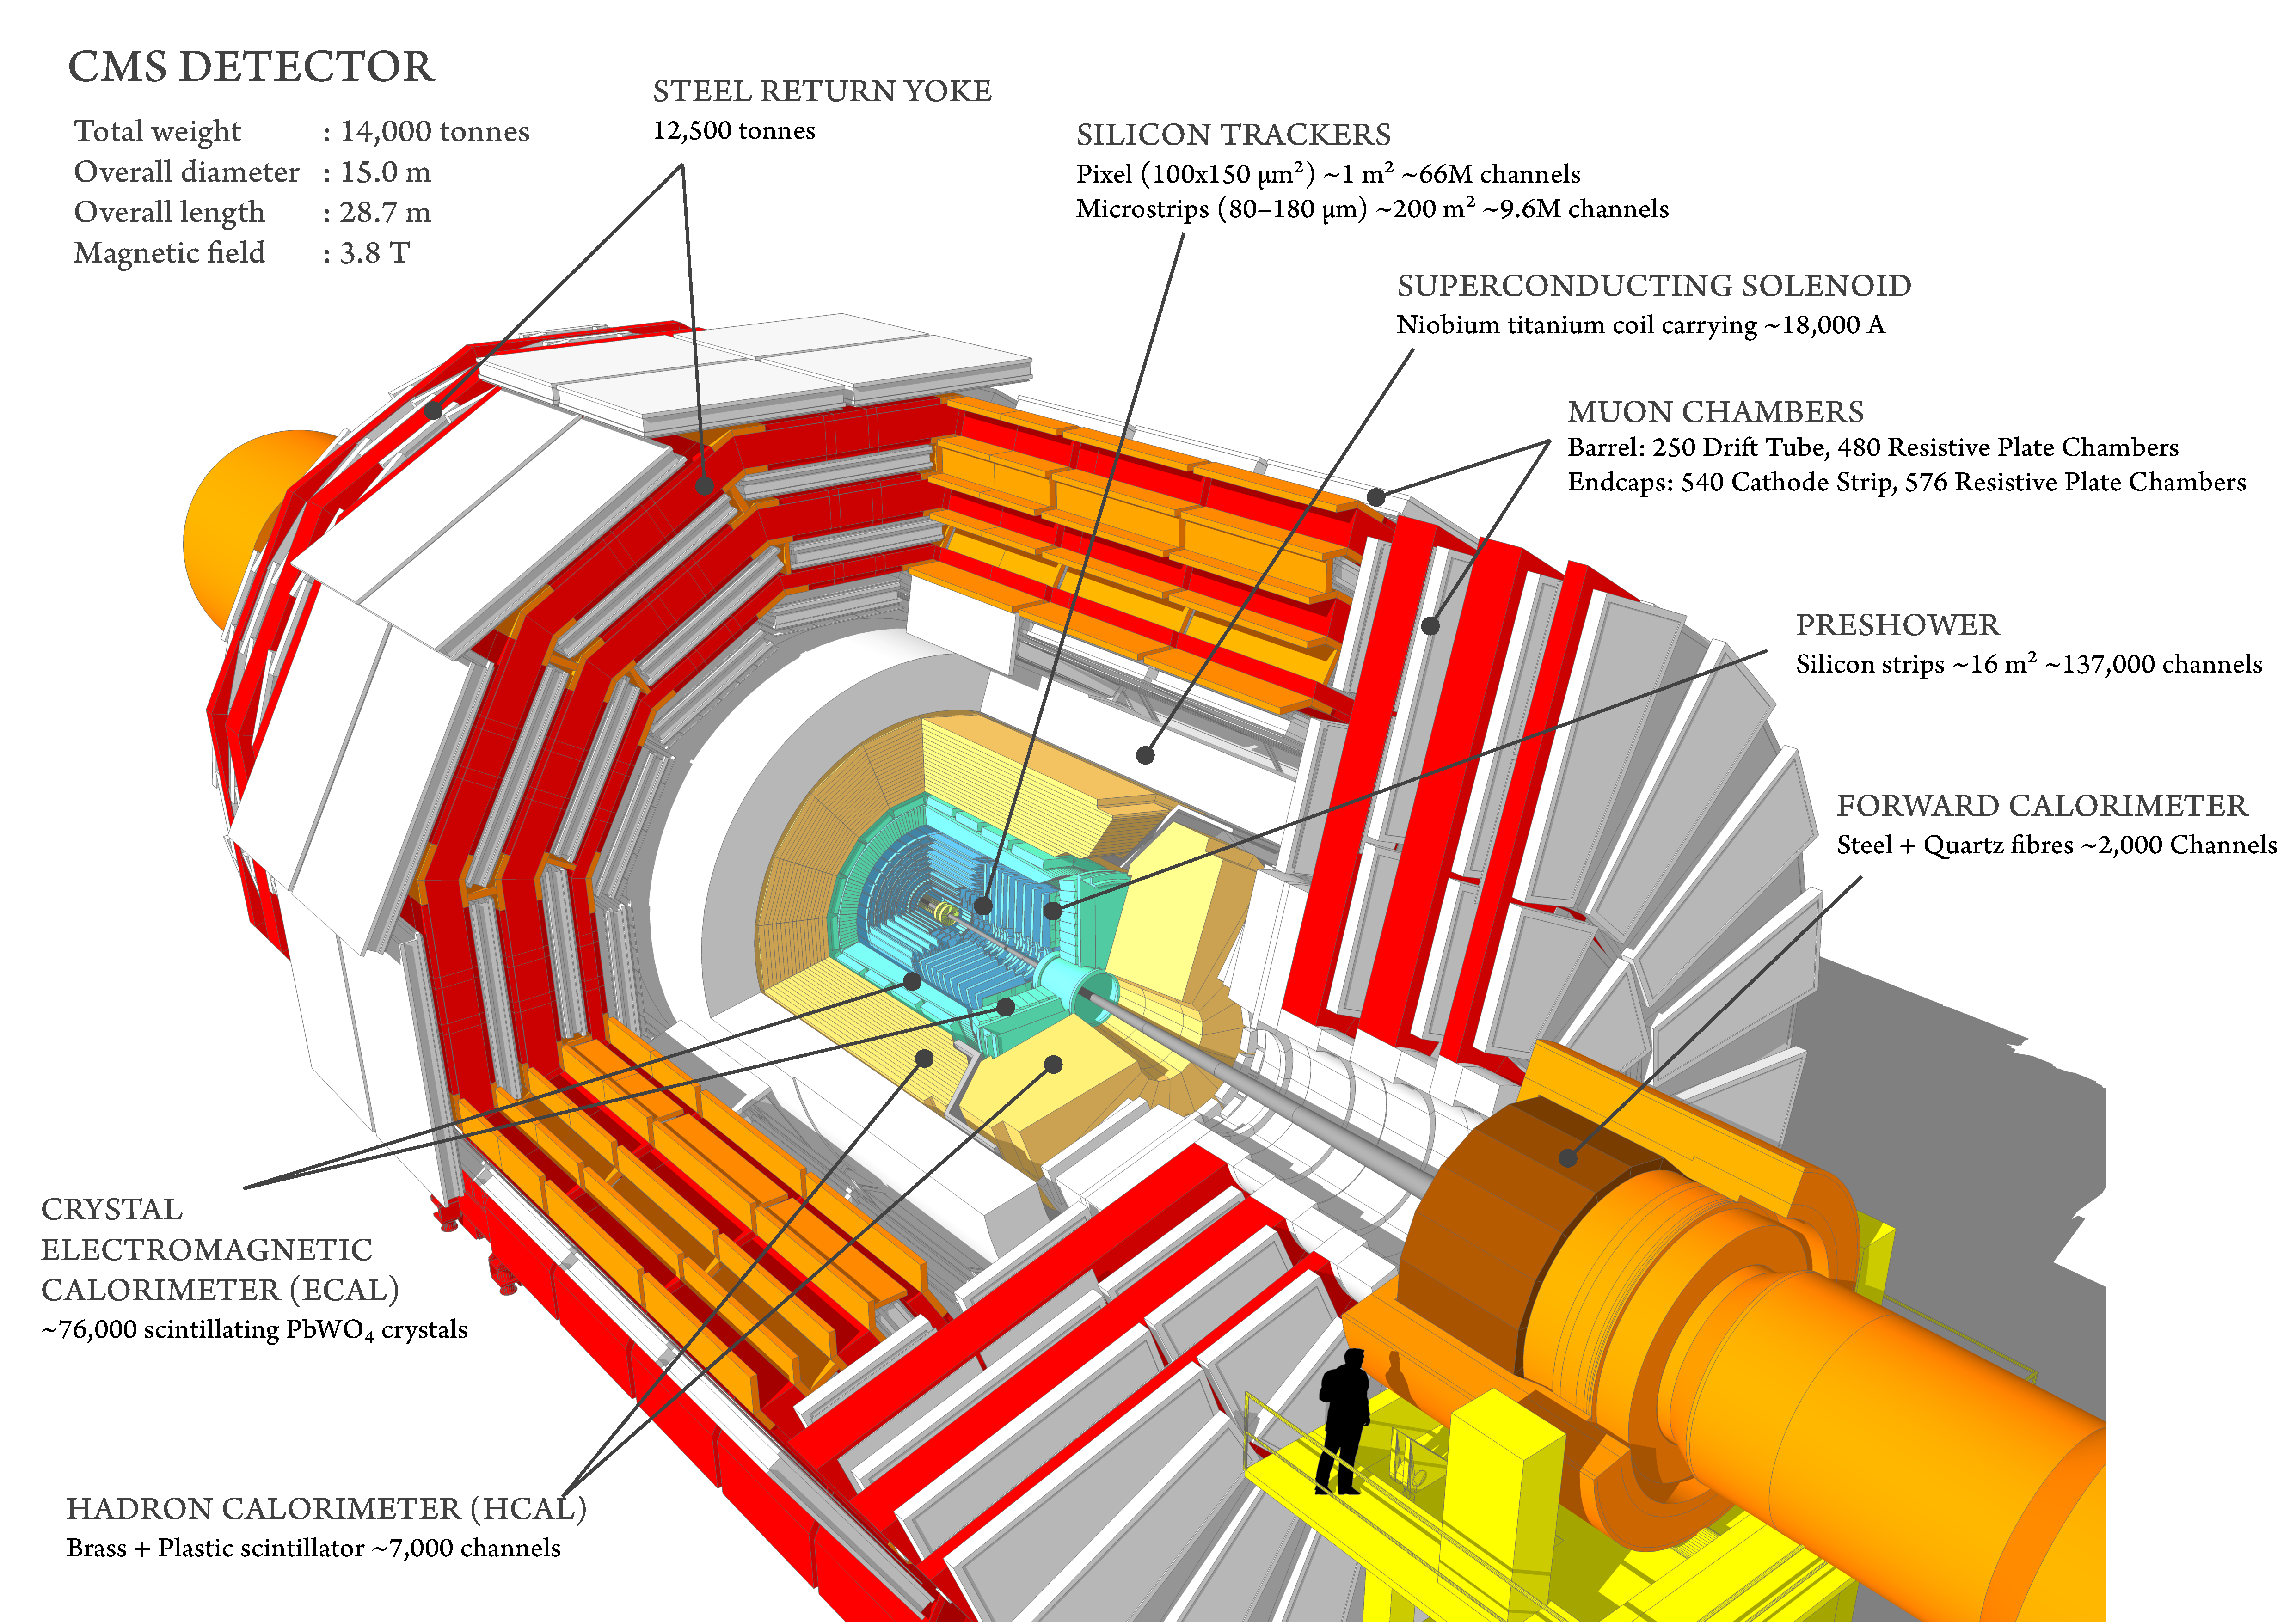
\includegraphics[width=0.99\mylength]{resources/CMS_cutaway_labels.pdf}
    \vspace*{-0.0cm}
    \caption{A cutaway view of the CMS detector. Figure from \cite{Sakuma:2013jqa}.}
    \label{fig:CMS_cutaway}
    \vspace*{-0.3cm}
\end{figure}

\begin{figure}[!ht]
    \vspace*{-0.0cm}
    \centering
    \setlength{\mylength}{\textwidth}
    \includegraphics[width=0.85\mylength]{resources/CMS_slice.png}
    \vspace*{-0.0cm}
    \caption{A slice of the CMS detector, with an illustration of the behaviour of different particles. Figure from \cite{Barney:2120661}.}
    \label{fig:CMS_slice}
    \vspace*{-0.3cm}
\end{figure}

The coordinate system in CMS has its origin centered at the nominal collision point within the detector. The $z$-axis follows the beam line, the $y$-axis points vertically upward, and the $x$-axis points radially inward toward the center of the LHC ring. The azimuthal angle $\phi$ is measured from the $x$-axis in the $x-y$ plane, with the radial coordinate denoted as $r$, and the polar angle $\theta$ is measured from the $z$-axis. However, $\theta$ is not often used because it is not Lorentz invariant for boosts along the direction of the beam. Instead, the pseudorapidity is defined as $\eta = -\ln{\left(\tan{\frac{\theta}{2}}\right)}$, which is Lorentz invariant. From this, it is possible to define the momentum orthogonal to the beam direction, denoted as $p_T$.

The silicon tracker is designed to measure the trajectory, charge and momentum of charged particles traversing it, as well as to reconstruct secondary vertices. It comprises two types of silicon detectors: the pixel detector (inner tracker) and the silicon strip tracker (outer tracker). They operate by measuring the ionization of charged particles. When a charged particle traverses the doped silicon wafer, it creates electron-hole pairs that move toward collection electrodes due to an applied electric field. These pairs are organized into silicon strips or pixels, providing a two-dimensional measurement. Multiple silicon wafers are arranged in different layers, and the hits measured in each layer are used to reconstruct the tracks of charged particles through the detector. The pixel detector is the innermost component, consisting of four barrel layers and three endcap disks. The silicon strip tracker is positioned just outside, extending to a radius of 1.1 m and comprising 15148 strips arranged in ten barrel layers and twelve endcap disks.

The primary purpose of the electronic calorimiter (ECAL) is to measure the energy and direction of electrons, positrons and photons. It is constructed with homogeneous lead tungstate (PbWO$_4$) crystals that serve as both active scintillating material to detect the electromagnetic signal and absorbing material to initiate electromagnetic (EM) showers. Energy deposition is measured through crystal ionization, and their deexcitation photons are detected by dedicated photodetectors. The short radiation length of the crystals, $X_0 = 0.89$ cm, ensures that the EM showers remain confined within a small region. The photodetectors are designed to withstand the high radiation and high magnetic field environment while being sufficiently fast compared to the LHC bunch crossing time. The ECAL consists of main parts: the ECAL barrel (EB), covering $\abs{\eta} < 1.479$, composed of 61200 crystals and which uses avalanche photodiodes, and the ECAL endcaps (EE), covering $1.479 < \abs{\eta} < 3.0$, composed of 7324 crystals in each (lower granularity compared to the barrel) and which use vacuum phototriodes. To account for the reduced endcap granularity, preshower detectors are installed before the lead tungstate crystals, covering $1.653 < \abs{\eta} < 2.6$, intended for identifying neutral pions, distinguish electrons against minimum ionizing particles, and improve position measurements. This design enables the ECAL to completely stop electrons and photons emerging from the tracker, allowing for accurate energy measurement.

Four hadronic calorimeters (HCAL) are positioned outside the ECAL. They are designed to generate hadronic showers when strongly interacting particles pass through their absorption material. These particles interact in the absorber layers, producing numerous secondary particles and often showers, which are measured by the scintillators. The HCAL are bigger than the ECAL because the nuclear interaction length $\lambda_\text{int}$ is also larger than the electromagnetic radiation length $X_0$ (e.g., for iron, $\lambda_\text{int}=16.8$ cm, while $X_0=1.76$ cm \cite{Buckley:2021fcn}). The HCAL barrel (HB) rests between the ECAL and the magnet ($R=1.77-2.95$ m), covering $\abs{\eta} < 1.4$. The HCAL endcap (HE) covers $1.3 < \abs{\eta} < 3.0$. Both the HB and the HE are made of brass and plastic scintillators. The HCAL outer detector (HO) is placed outside the magnet in the barrel region ($\abs{\eta} < 1.26$) to catch the tail of the shower, and it is made of iron and plastic scintillators. To ensure optimal efficiency in different pseudorapidity ranges, there is a fourth HCAL placed in the endcap regions after the muon systems. The HCAL forward detector (HF) covers $3.0 < \abs{\eta} < 5.0$ at $\abs{z} = 11.2$ m, where it is subject to much higher radiation. It is distinguished from the other HCAL sections because it is built with steel and quartz fibers, leading to shorter hadronic showers for better absorption of very forward hadron showers. Note that the ECAL already absorbs a fraction of the energy of the hadrons, but the HCAL design allows it to fully stop the hadrons and measure any remaining energy, which is later combined with the ECAL information to obtain a complete picture.

Muon identification was a focal point for CMS because muons produced in proton-proton collisions offer clear lepton signatures for a wide range of physics processes and helps with their reconstruction. The CMS muon system consists of several subdetectors dedicated to measure muons with high precision. To achieve accurate muon identification, the muon detectors were designed with extensive pseudorapidity coverage, up to $\eta = 2.4$. CMS's muon system uses three types of detectors: Drift Tubes, Resistive Plate Chambers and Cathode Strip Chambers. Muon Drift Tubes (DT) contain a wire and a gas mixture (85\% Ar, 15\% CO$_2$) at atmospheric pressure that ionizes when traversed by a muon. The deexcitation electrons follow the electric field to reach the wire, recording the signal. By recording the distance from the wires and the location along the wires, the DTs determine two coordinates of the muon's positions. Resistive Plate Chambers (RPC) are gaseous (95.2\% C$_2$H$_2$F$_4$, 4.5\% i-C$_4$H$_{10}$, 0.3\% SF$_6$) parallel plate capacitors with high timing resolution. Cathode Strip Chambers (CSC) consist of positively charged anode wires crossed with negatively charged cathode panels within a gas volume (40\% Ar, 50\% CO$_2$, and 10\% CF$_4$), which ionize when traversed by a muon: positive ions move toward the cathode and the electrons move toward the anode wires. In the CMS detector's barrel ($\abs{\eta} < 1.2$), the DTs are arranged in four concentric layers interleaved with five layers of the iron magnet yoke and six layers of RPCs, as shown in Figure \ref{fig:CMS_slice}. In the endcap region, reaching $\eta = 2.4$, there are three RPC layers (up to $\eta = 1.6$) and six CSC layers, chosen in this region for their ability to resist high non-uniform magnetic fields. Muons do not deposit much energy in matter, so they pass through both calorimeters with most of their momentum. The muon chambers then provide further information about the muon's trajectory, as they are the only particles with a clear signal in this section. These trajectories, combined with those of the trackers, allow for better muon identification and provide additional data on their momenta.

Storing all recorded events in the detector is impractical, so only events meeting specific conditions are preserved. The Level 1 (L1) Trigger uses local trigger information from all subdetectors, excluding the Inner Tracker, to determine whether to save an event. With the aid of custom hardware and firmware, it reduces the event rate from 40 MHz to 100 kHz. It considers information from the four highest $E_T$ electrons, photons, central jets, forward jets, tau-jets, the four highest $p_T$ muons, the event's missing transverse energy (MET), and the scalar sum of the jet transverse momenta (HT). Subsequently, data is processed by the High-Level Trigger (HLT), a comparatively slower software, to further filter events based on trigger menus, reducing the rate to around 1 kHz. The CMS offline physics object reconstruction is achieved using the Particle Flow (PF) algorithm, which integrates information from all subdetectors to reconstruct all particles in the event.

The Compact Muon Solenoid experiment is one of the largest international scientific collaborations in history, involving more than 6000 particle physicists, engineers, technicians, students and support staff from 257 institutes in 59 countries as of October 2023 \cite{CERN:CMS_people}.

\section{The discovery of the Higgs boson}

Nearly 50 years after the Higgs boson had been proposed, in 2012, the CMS and ATLAS collaborations observed a new scalar boson with a mass of 125 GeV \cite{CMS:2012qbp, ATLAS:2012yve}. The properties of this particle were compatible with those of the Higgs boson, including its spin and mass (in 2012 precision electroweak measurements and direct searches at LEP had constrained the mass of the Higgs boson to be in the interval $114.4\ \GeV < m_H < 152\ \GeV$ at 95\% conficende level (CL) \cite{ALEPH:2010aa, LEPWorkingGroupforHiggsbosonsearches:2003ing}).

\begin{figure}[!ht]
    \vspace*{-0.0cm}
    \centering
    \setlength{\mylength}{\textwidth}
    \includegraphics[width=0.60\mylength]{resources/CMS_Higgs_diphoton.jpg}
    \vspace*{-0.0cm}
    \caption{The diphoton invariant mass distribution computed by CMS in \cite{CMS:2012qbp}. The lines represent the fitted background and signal, and the coloured bands $\pm1\ \sigma$ and $\pm2\ \sigma$ in the background estimate.}
    \label{fig:CMS_Higgs_diphoton}
    \vspace*{-0.3cm}
\end{figure}

The CMS experiment used data recorded at $\sqrt{s} = 7$ and 8 TeV, with integrated luminosities of up to 5.1 fb$^{-1}$ at 7 TeV and 5.3 fb$^{-1}$ at 8 TeV. For the search, five decay modes were employed: H$\decaysto\gamma\gamma$, $ZZ^*$, $WW^*$, $\tau^+\tau^-$ and $b\bar{b}$, which according to the SM is about 89\% of all the decay modes of the Higgs boson (see Table \ref{tab:Higgs_decays}). They reported an excess of events over the expected background, consistent with the production of a new particle with mass near 125 GeV, with an observed local signigicance of 5.0 standard deviations ($\sigma$). The strongest evidence came from the two final states with the best mass resolution, which are H$\decaysto\gamma\gamma$ with a significance of 4.1$\sigma$ and H$\decaysto ZZ^*$ with a significance of 3.2$\sigma$. Moreover, H$\decaysto\gamma\gamma$ indicated that the new particle was a boson with spin different from one \cite{CMS:2012qbp}. Figure \ref{fig:CMS_Higgs_diphoton} presents the diphoton invariant mass $m_{\gamma\gamma}$ presented by CMS in 2012, where the excess at 125 GeV is evident in the weighted and unweighted distributions.

The confidence level of the combined result as a function of the Higgs boson mass is presented in Figure \ref{fig:CMS_Higgs_CLs}. The observed values are shown as the solid points, while the dashed line represents the median of the expected results for the background-only hypothesis. The green and yellow bands indicate the ranges where CLs values are expected to lie in 68\% and 95\% of the experiments under the background-only hypothesis. The red horizontal lines indicate CLs values of 0.05, 0.01, and 0.001. The mass regions where the observed CLs values are below these lines are excluded with the corresponding (1 - CLs) confidence levels. In the range $121.5 < m_H < 128$ GeV a significant excess is observed, and the SM Higgs boson cannot be excluded at 95\% CL. They also determined the Higgs boson mass by using the $\gamma\gamma$ and $ZZ^*$ decay modes, obtaining a value of $m_H=125.3\pm0.4\text{ (stat.)}\pm0.5\text{ (syst.)}\ \GeV = 125.3\pm0.6\ \GeV$.

\begin{figure}[!ht]
    \vspace*{-0.0cm}
    \centering
    \setlength{\mylength}{\textwidth}
    \includegraphics[width=0.60\mylength]{resources/CMS_Higgs_CLs.jpg}
    \vspace*{-0.0cm}
    \caption{The CLs values for the SM Higgs boson hypothesis as a function of the Higgs boson mass in the range 110-145 GeV, by CMS in \cite{CMS:2012qbp}.}
    \label{fig:CMS_Higgs_CLs}
    \vspace*{-0.3cm}
\end{figure}

In ATLAS analysis \cite{ATLAS:2012yve}, they reported a significance of 5.9$\sigma$ and a mass of $m_H=126.0\pm0.4\text{ (stat.)}\pm0.4\text{ (syst.)}\ \GeV = 126.0\pm0.6\ \GeV$, compatible with CMS's results.
\chapter[Analysis]{Analysis}

This chapter is the central cornerstone of this dissertation. In it, we will discuss the analysis conducted, starting with a general overview, followed by an explanation of the samples, triggers, and object definitions. We will then discuss the corrections made to the data and simulations to enhance the analysis results. We will also cover the various criteria utilized in event selection and how the signal and background have been modeled. Ultimately, we will present the expected limits for each channel. The chapter concludes by addressing the subsequent steps required prior to data unblinding and the attainment of the final experimental measurement.

\section{Analysis overview}

\section{Samples and triggers}

\todo{Explain data, background and signal MC simulation, triggers}

\section{Object definitions}

\todo{Primary vertex, leptons?, jets, missing energy, photons, mesons}

\section{Corrections to data and simulations}

\todo{Pileup reweighting, L1 prefiring corrections, photon scale and resolution, photon mvaid efficiency, Lepton ID reconstruction efficiency and energy scale (?), meson reconstruction (+regression of the pt), triggers scale factors}

\section{Event selection}

\todo{Gluon fusion selection for each channel}

\section{Signal and background modelling}

\todo{signal, background model from MC and data, bias studies}

\section{Results}

\section{Multivariate analysis for final results}

\todo{talk about MVA and what are next steps before unblinding data}



\phantomsection
\addcontentsline{toc}{chapter}{Conclusions}
\chapter*{Conclusions}

These are the conclusions of the project.

\clearpage{\thispagestyle{empty}}




\appendix
\phantomsection
\addcontentsline{toc}{chapter}{Appendix}
\chapter{Appendix}\label{chap:appendix}

\section{BDT regression models}\label{sec:appendix_models}

In Section \ref{sec:meson_reconstruction} the Boosted Decision Trees used to improve the reconstruction of each full meson's transverse momentum were introduced. The hyperparemeters for these models are shown in Table \ref{tab:hyperparameters_models}, for each channel.

\begin{table}[!ht]
    \begin{lrbox}{\verbbox}
        \footnotesize
        \verb+TMVA::Types::kBDT+
    \end{lrbox}
    \centering
    \begin{tabular}{|l|C{2.45cm}|C{2.45cm}|C{2.45cm}|C{2.45cm}|}
        \hline
        \cellcolor{lightgray}Hyperparameter & \cellcolor{lightgray}$\phi$ & \cellcolor{lightgray}$\omega$ & \cellcolor{lightgray}$D^{*0}$ 2-body & \cellcolor{lightgray}$D^{*0}$ 3-body \\ \hline
        \verb+VarTransform+         &G, N, P&G, P, D&D, G   &    \\
        \verb+NTrees+               &1000   &1500   &1400   &    \\
        \verb+BoostType+            &Grad   &Grad   &Grad   &    \\
        \verb+Shrinkage+            &0.045  &0.066  &0.044  &    \\
        \verb+MaxDepth+             &6      &4      &6      &    \\
        %\verb+SeparationType+       &RegressionVariance&RegressionVariance&RegressionVariance&    \\
        \verb+nCuts+                &38     &25     &19     &    \\
        \verb+UseRandomisedTrees+   &True   &True   &False   &    \\
        \verb+UseNvars+             &76     &28     &57     &    \\
        \verb+UseBaggedBoost+       &False  &False  &False   &    \\
        \verb+BaggedSampleFraction+ &1.203  &0.880  &1.464 &    \\
        \verb+PruneMethod+          &NoPruning&NoPruning&ExpectedError&    \\
        \verb+PruneStrength+        &-      &-      &26     &    \\
        \verb+PruningValFraction+   &-      &-      &0.689 &    \\
        \hline
        \end{tabular}
    \caption{Hyperparameters of the BDTs regressing the transverse momentum of each meson. These parameters are available options for the \usebox{\verbbox} regressor. Each option is described in detail in Ref. \cite{TMVA:2007ngy}.}
    \label{tab:hyperparameters_models}
\end{table}


%%%%%%%%%%%%%%%%%%%%%%%%%%%%%%%%%%%%%%%%%%%%%%%%%%%%%%%%%%%%%%%%%%%%%%%%%
\backmatter
\phantomsection
%\include{mainmatter/999_biblio}
\selectlanguage{english}
\addcontentsline{toc}{chapter}{References}
\bibliographystyle{JHEP}
\bibliography{mainmatter/999_citations}



\end{document}
